\subsubsection{BinarySearchTree}
The solution checker is designed to check that the tree object created from the students drawing, matches the tree created in the solution. The solution checker will recursively call a function named checkNode that will compare each node in the tree with the corresponding node in the solution. If the two nodes does not match, the solution checker will return false, and the student will have answered incorrect. If all nodes compared match the solution, the solution checker will return true, meaning that the student has answered the question correctly. The solution checker traverses the tree inorder. It will first check the left node, then the parent, then the right node. This solution checker is also used for AVL trees.
\\[11pt]
A function createBinarySearchTreeSolution was implemented to create a BST based on given arguments and/or existing tree object. This function was implemented so that the admin didn't need to manually create the solution trees for each question. The function takes an array with integers and possibly an existing tree as parameters. If the existing tree is not given, the function will create a new tree based on the values in the array. If the an existing tree is given, the values in the array is added to this tree. Its important to note that the function will not work with duplicate values in the array or given tree.
\\[11pt]
The createBinarySearchTreeSolution also needed to create resulting trees upon deleting an existing node in a tree. Because there are multiple ways to choose nodes for replacements when deleting a node with 2 children. It was required for the createBinarySearchTreeSolution to create a list of potential final resulting trees. It is required to specify whether the user wants to add nodes or remove nodes from the tree when creating the solution trees. The function cannot switch between the two during execution, and an existing tree is required in order to remove nodes in the tree.\cite{BinaryTree}\\[11pt]
The createBinarySearchTreeSolution will return an array containing the different states of the BST during its creation. Since there can be different resulting tree when deleting a parent node, all resulting trees will be stored in the array. The last element in the array will be the finished BST tree object that will be compared with the drawn tree from the students. Originally the drawn tree from the student will be a graph object and has to first be transformed into a tree class object using the general tree function "createTreeObjectFromCanvasObjectver1".Once transformed into a bst object the students tree will be compared with the all trees in the solution object in the solution checker mentioned earlier.
\begin{figure}[H]
	\centering
	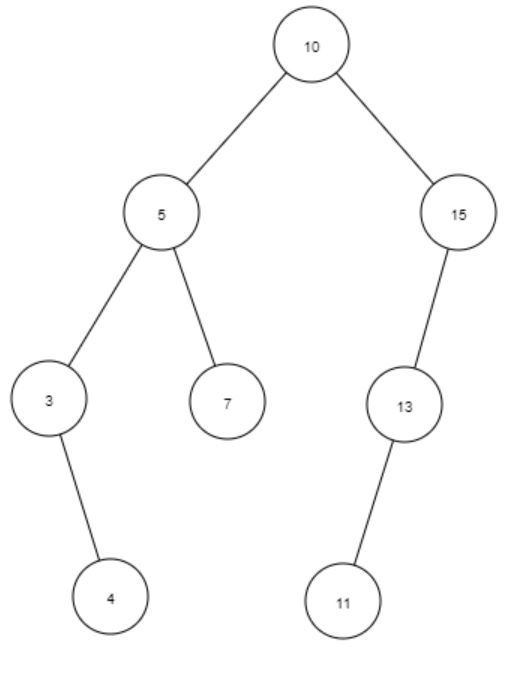
\includegraphics[width=250px, height=250px]{/trees/BST}
	\caption{The figure shows an example of a Binary Search Tree.}	
	\label{fig:BST}
\end{figure}
